% !TEX root = cha-soa.tex
\documentclass[../../main.tex]{subfiles}

\begin{document}

\section{Polymetric Views}

In 2003, Lanza and Ducasse introduced \emph{polymetric views}, a lightweight software visualization technique for reverse engineering and program comprehension \citebibliography{Lanz2003a}. It is based on two-dimensional graphs, where nodes represent software entities, such as classes or methods, and edges represent their relationships. A polymetric view adds information to these graphs by mapping up to five software metrics to visual properties of each node: width, height, position ($X, Y$), and color (using a grayscale from white to black). These metrics are directly derived from the source code rather than being computed by combining other metrics. For example, they can describe different aspects of a class, method, or attribute. Class metrics include the number of methods (NOM), the number of attributes (NOA), and the number of immediate subclasses (NOC). Method metrics include lines of code (LOC), the number of parameters (NOP), and the number of statements (NOS). Attribute metrics include the number of direct accesses from outside the class (NGA) and from within the class (NLA). The authors defined several predefined views at different levels of detail, while also allowing developers to create custom views. This approach helps developers assess the overall structure and quality of a system, locate important components, and identify unusual entities that may need refactoring or further analysis. An example of a polymetric view is shown in \figref{fig:polymetricView}.

\begin{figure}[h]
    \centering
    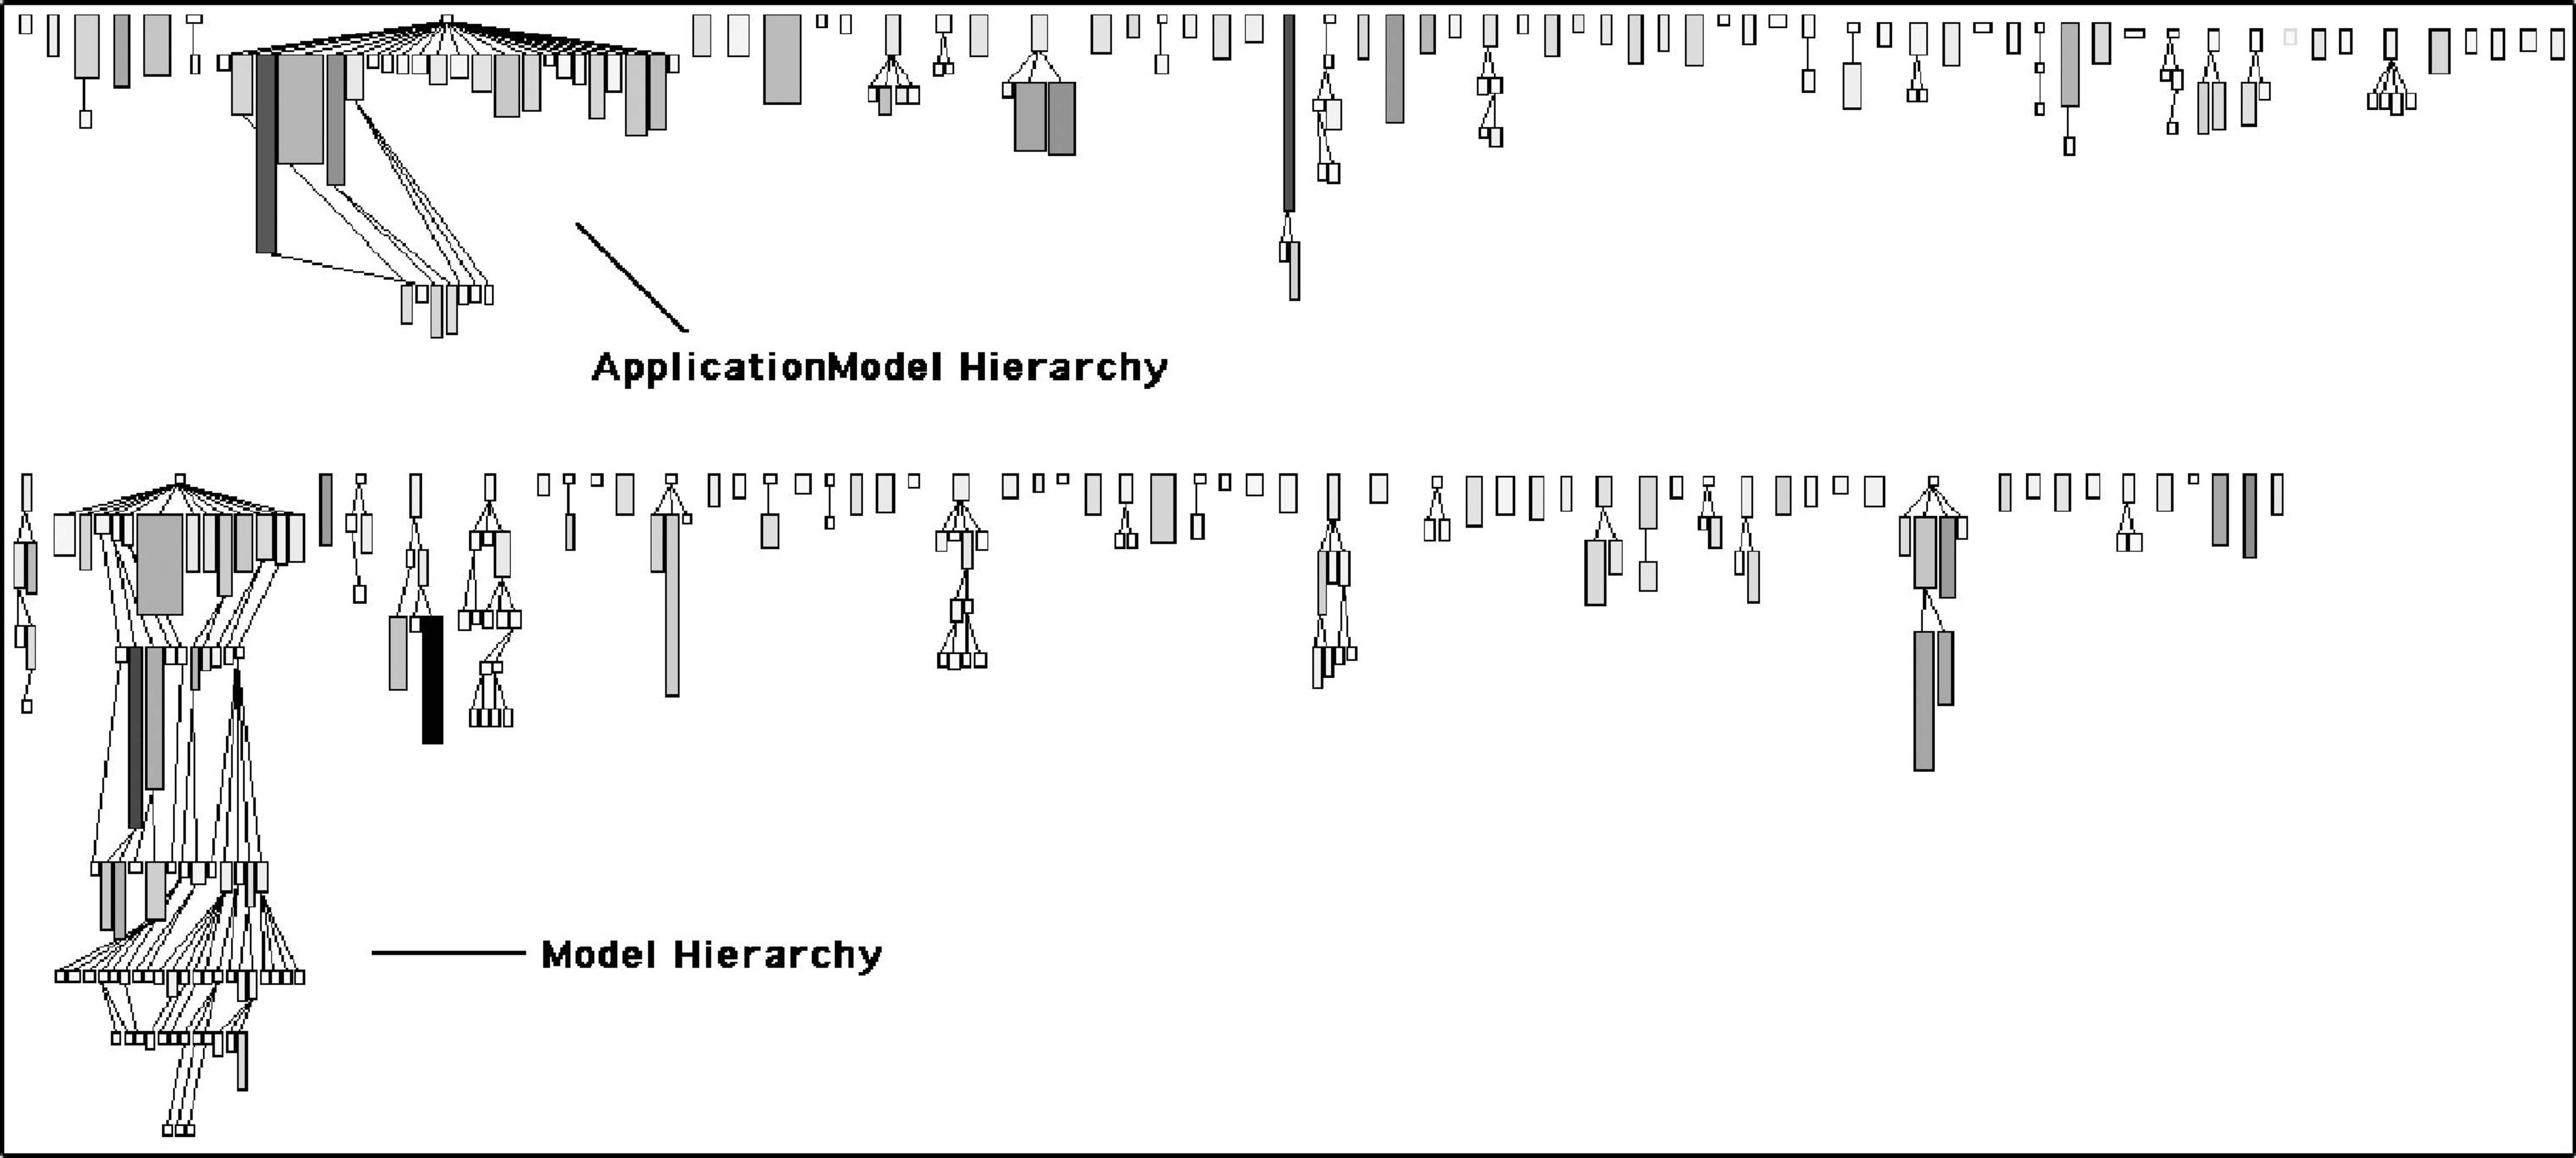
\includegraphics[width=\linewidth]{figures/soa/polymetricView}
    \caption[Example of a Polymetric View]{Example of a Polymetric View~\citebibliography{Lanz2003a}.}
    \label{fig:polymetricView}
\end{figure}

In 2022, Agouf~\etal~\citebibliography{Agou2022a} introduced \emph{Class Blueprint V2}, an evolution of the original Class Blueprint polymetric view \citebibliography{Lanz2003a}. The original Class Blueprint was designed to help developers understand the structure of a class, but it had some limitations. It did not show whether a method was covered by tests, did not identify dead code, did not clearly distinguish between class-side and instance-side methods, and did not show cyclomatic complexity. Class Blueprint V2 addresses these limitations by enhancing the original layout. Horizontally, the visualization is divided into three layers: the class side at the top, the instance side in the middle, and a bottom layer, called the ``cemetery'', for dead methods and unused attributes. Vertically, instance methods are organized into different groups. These include methods responsible for object creation, methods that compose the external interface of the class, and methods used internally by the class itself. Getter and setter methods are also placed close to the attributes they access to reduce the space usage. The visualization also uses colors and visual annotations to provide additional information. For example, tested methods have their upper third colored in green, attributes accessed by at least one subclass are shown in dark blue, while other attributes are shown in dark green. Different colors are also used for methods, such as brown for overriding methods and pale orange for overridden methods. Methods with high cyclomatic complexity are highlighted with a red border. These visual elements allow developers to quickly identify potentially problematic methods and attributes. In particular, the detection of dead code was the most appreciated feature, as it can reveal code that developers forgot to remove. An example of Class Blueprint V2 is shown in \figref{fig:bluePrintV2}.

\begin{figure}[h]
    \centering
    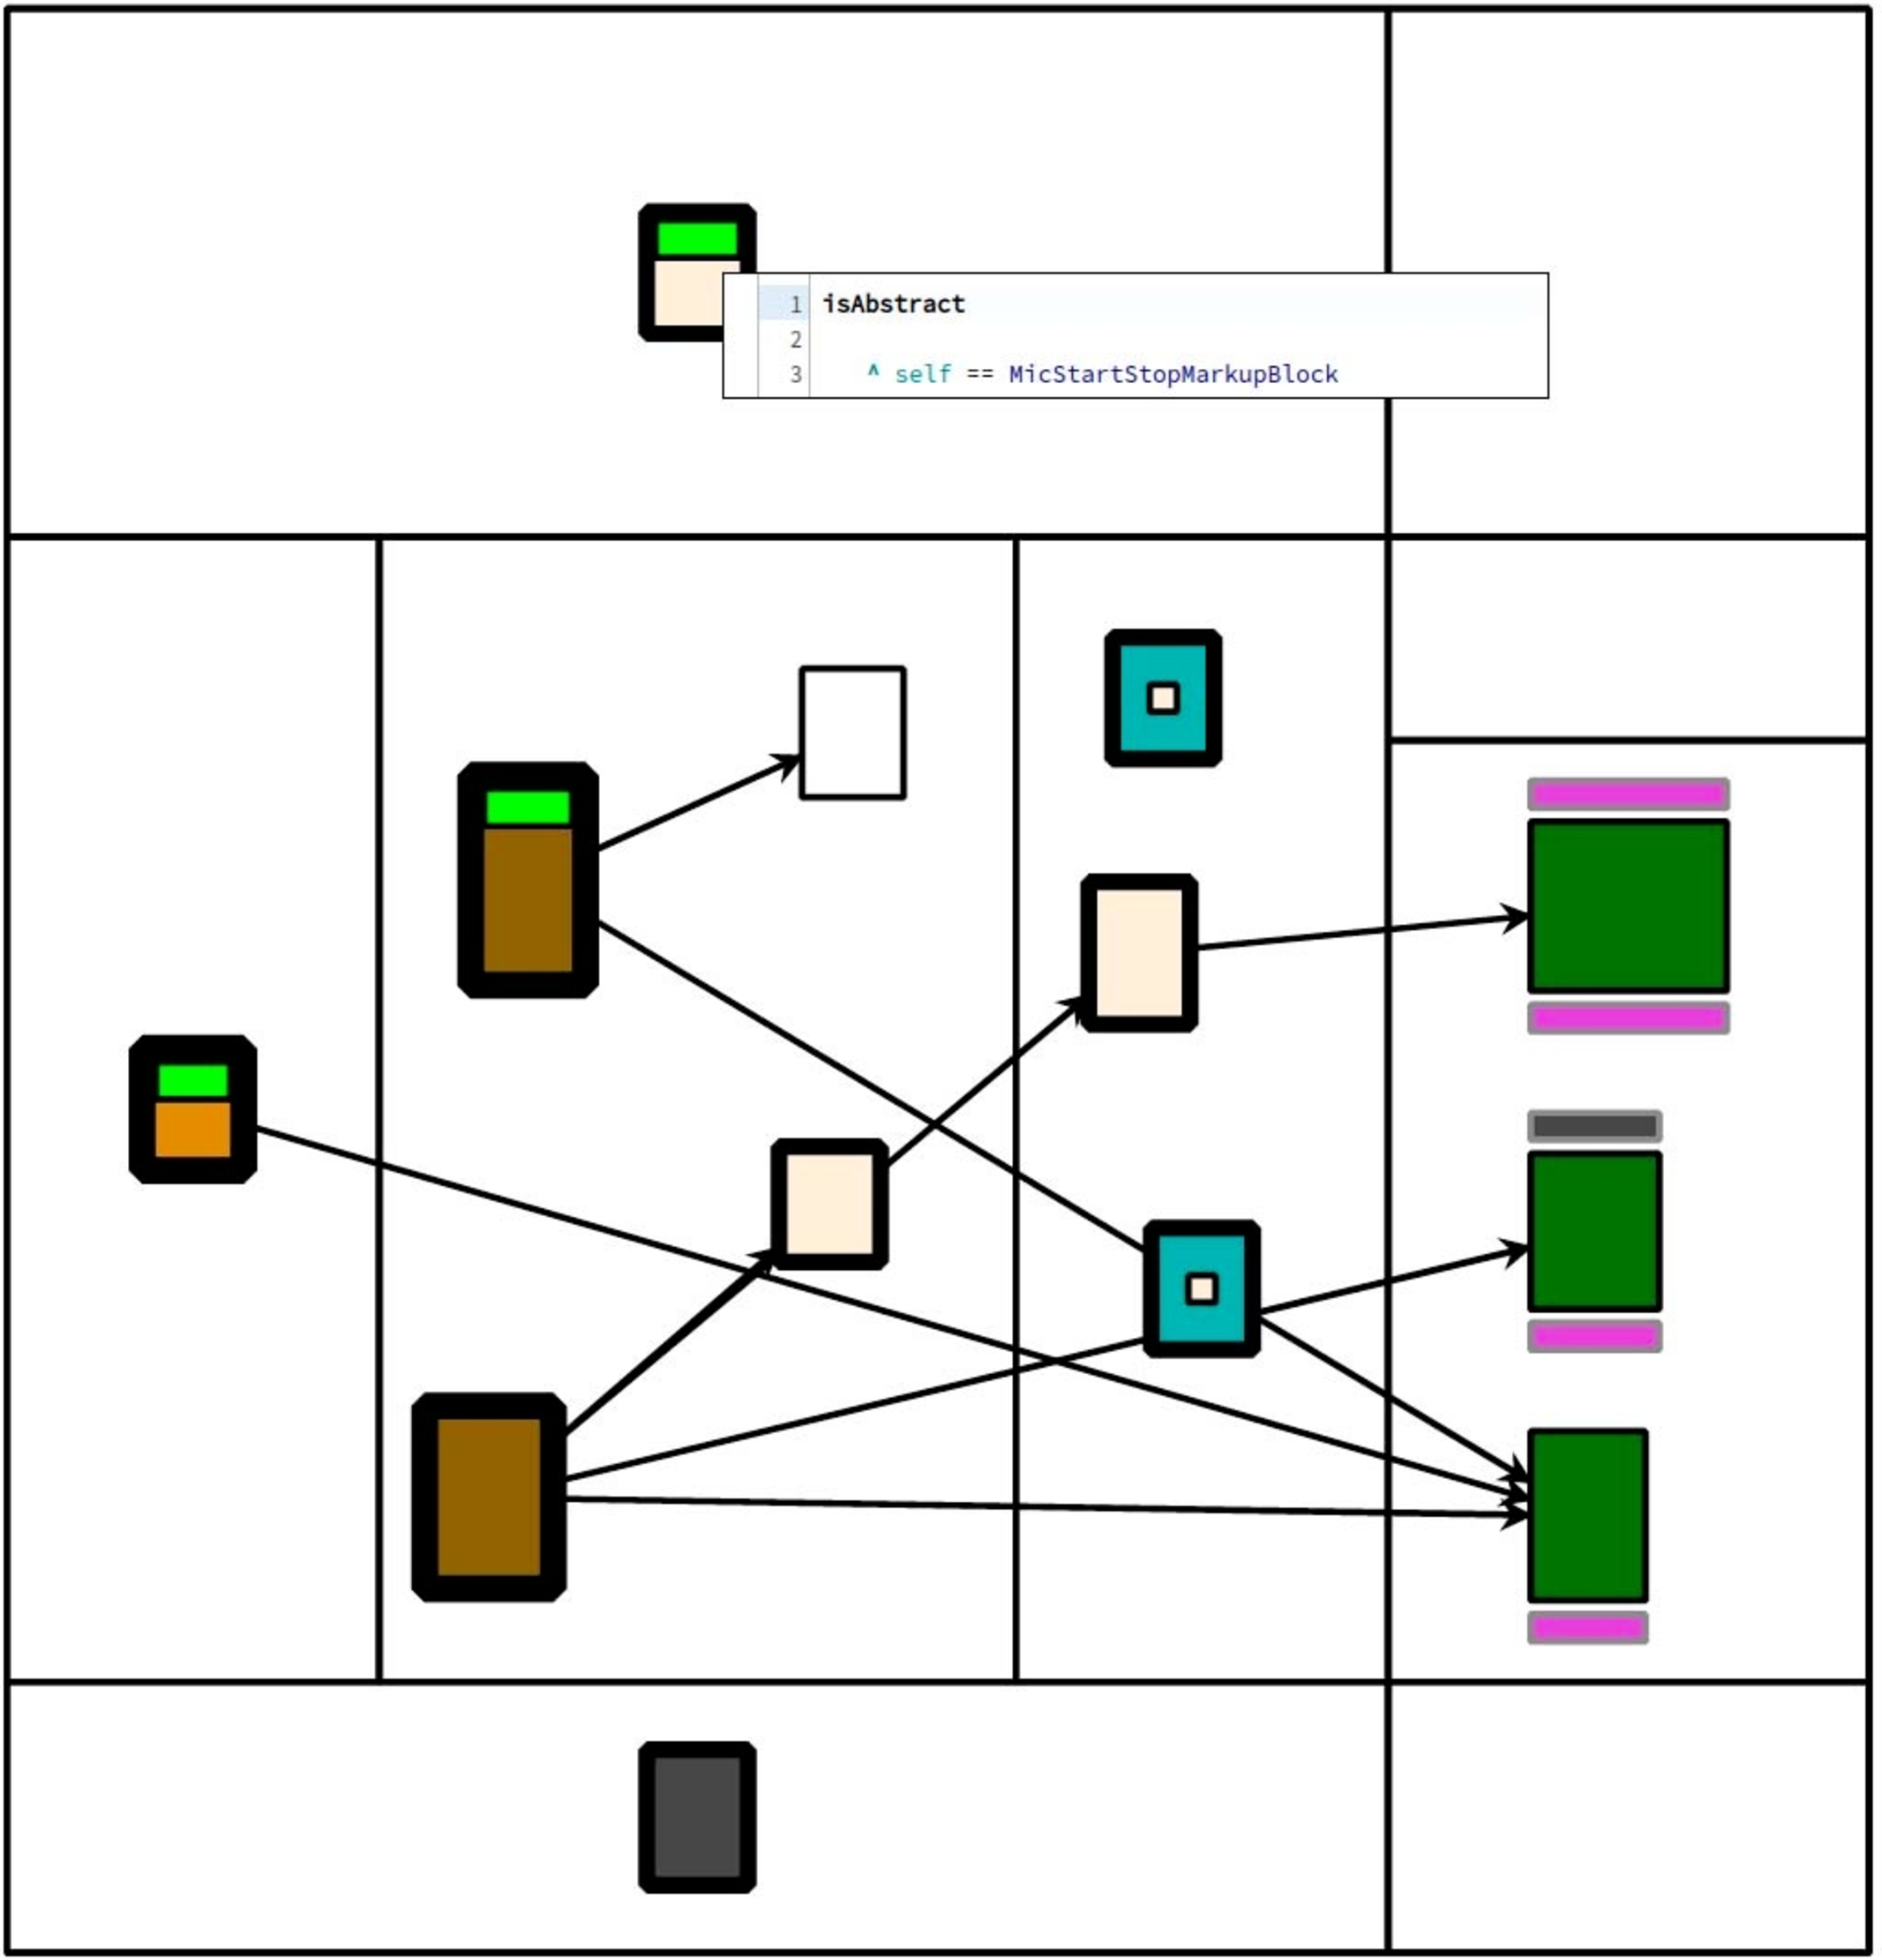
\includegraphics[width=0.65\linewidth]{figures/soa/bluePrintV2}
    \caption[Example of a Class Blueprint V2]{Example of a Class Blueprint V2~\citebibliography{Agou2022a}.}
    \label{fig:bluePrintV2}
\end{figure}

\end{document}